\documentclass[a4paper,oneside,DIV=12,12pt,headings=normal]{scrartcl}

%%% Length calculations
\usepackage{calc}
%%%

%%% Support for color
\usepackage{xcolor}
\definecolor{lightblue}{HTML}{03A9F4}
\definecolor{red}{HTML}{F44336}
%%%

%%% Graphics inclusion
\usepackage{graphicx}
%%%

%%% Font selection
\usepackage{fontspec}

\setromanfont{STIX Two Text}[
	SmallCapsFeatures = {LetterSpace = 5},
]

\setsansfont{Source Sans Pro}[
]

\setmonofont{Source Code Pro}[
]
%%%

%%% Math settings
\usepackage{amsmath,unicode-math}
\setmathfont{STIX Two Math}

\usepackage{IEEEtrantools}
\usepackage{mleftright}
%%%

%%% Font settings for different KOMA Script elements
\setkomafont{pagenumber}{\rmfamily}
\setkomafont{disposition}{\rmfamily\bfseries}
%%%

%%% Typographic enhancements
\usepackage{microtype}
%%%

%%% Language-specific settings
\usepackage{polyglossia}
\setmainlanguage{ukrainian}
%%%

%%% List settings
\usepackage{enumitem}
\setlist[enumerate]{
	leftmargin = *,
}
%%%

%%% Captions
\usepackage{caption}
\usepackage{subcaption}

\DeclareCaptionLabelFormat{closing}{#2)}
\captionsetup[subtable]{labelformat = closing}
\captionsetup[subfigure]{labelformat = closing, position = auto}
%%%

%%% Tables
\usepackage{booktabs}
\usepackage{longtable}

\usepackage{multirow}

\usepackage{array}
\newcolumntype{v}[1]{>{\raggedright\arraybackslash\hspace{0pt}}p{#1}}
\newcolumntype{b}[1]{>{\centering\arraybackslash\hspace{0pt}}p{#1}}
\newcolumntype{n}[1]{>{\raggedleft\arraybackslash\hspace{0pt}}p{#1}}

\usepackage{kbordermatrix} % labeling array indices
%%%

%%% Floats on a single row
\usepackage{floatrow}
\newfloatcommand{capbtabbox}{table}[][\FBwidth]
%%%

%%% Links and hyperreferences
\usepackage{hyperref}
\hypersetup{
	colorlinks      = false,
	linkbordercolor = red,
	urlbordercolor  = lightblue,
	pdfborderstyle  = {/S/U/W 1.5},
}
%%%

%%% All caps
\newcommand{\allcaps}[1]{{\addfontfeatures{LetterSpace = 3}#1}}
%%%

\setlength{\emergencystretch}{1em}

\begin{document}
	\hyphenation{муль-ти-плек-со-рів де-муль-ти-плек-со-рів}
	\begin{titlepage}
	\centering
		Міністерство освіти і науки України\\
		Національний авіаційний університет\\
		Навчально-науковий інститут комп'ютерних інформаційних технологій\\
		Кафедра комп'ютеризованих систем управління

		\vspace*{\fill}

		Лабораторна робота №3\\
		з дисципліни «Комп'ютерна схемотехніка»\\
		на тему «Дослідження компараторів та схем контролю»

		\vspace*{\fill}
		
		\begin{flushright}
			Виконав:\\
			студент ННІКІТ СП-225\\
			Клокун В.\,Д.\\
			Перевірив:\\
			Іскренко Ю.\,Ю.
		\end{flushright}

		Київ 2018
    \end{titlepage}
	
	\section{Мета роботи}
		Вивчення логіки роботи, принципів побудови й синтезу схем порівняння (компараторів) та контролю парності. Визначення основних характеристик схем порівняння й контролю парності на інтегральних мікросхемах.
	
	\section{Хід роботи}
		\subsection{Дослідження схеми порівняння чотирьохрозрядного слова~$A$ з~константою нуля}
			Перетворюємо умову рівності слова~$A$ константи нуля з виразу до вигляду, зручного для побудови на логічних елементах НЕ—І:
			\begin{equation}
			\label{eqn:eqn-01}
				F_{A = 0} = \neg \left( \neg \left( \neg A_4 \land \neg A_3 \land \neg A_2 \land \neg A_1 \right) \right).
			\end{equation}
			
			Збираємо схему порівняння на логічних елементах НЕ—І~(рис.~\ref{subfig:comparator-schematics-01-01}) відповідно до виразу~\eqref{eqn:eqn-01}. Подаємо на входи схеми порівняння різні двійкові набори~(табл.~\ref{tab:comparator-datasets-01}) і записуємо в цю ж таблицю значення функції~$F_{A = 0}$.
			
			\begin{figure}[!htbp]
			\centering
				\begin{subfigure}[c]{0.5\linewidth - 1em}
				\centering
					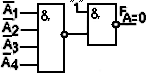
\includegraphics[height = 4\baselineskip]{./assets/01-01.png}
				\caption{}
				\label{subfig:comparator-schematics-01-01}
				\end{subfigure}
				~
				\begin{subfigure}[c]{0.5\linewidth - 1em}
				\centering
					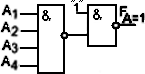
\includegraphics[height = 4\baselineskip]{./assets/01-02.png}
				\caption{}
				\label{subfig:comparator-schematics-01-02}
				\end{subfigure}
			\caption{Схеми порівняння}
			\label{fig:comparator-schematics}
			\end{figure}
			
			
			
			\begin{table}[!htbp]
			\centering
				\begin{tabular}{lrr}
					\toprule
						$A$ & $F_{A = 0}$ & $F_{A = 1}$\\
					\midrule
						1001 & & \\
						1011 & & \\
						0000 & & \\
						1110 & & \\
						1111 & & \\
					\bottomrule
				\end{tabular}
			\caption{Значення функцій порівняння}
			\label{tab:comparator-datasets-01}
			\end{table}
			
		\subsection{Дослідження схеми порівняння чотирьохрозрядного слова~$A$ з~константою одиниці}
			Перетворюємо умову рівності слова~$A$ константи одиниці до вигляду, зручного для побудови на елементах НЕ—І, аналогічно до виразу~\eqref{eqn:eqn-01}:
			\begin{equation}
			\label{eqn:eqn-02}
				F_{A = 1} = \neg \left( \neg \left( A_4 \land A_3 \land A_2 \land A_1 \right) \right).
			\end{equation}
			
			Збираємо схему порівняння на логічних елементах НЕ—І~(рис.~\ref{subfig:comparator-schematics-01-01}) відповідно до виразу~\eqref{eqn:eqn-02}. Подаємо на входи схеми порівняння різні двійкові набори~(табл.~\ref{tab:comparator-datasets-01}) і записуємо значення функції~$F_{A = 1}$.
			
		\subsection{Дослідження схеми порівняння двох чотирьохрозрядних слів~$A$ і~$B$ на~рівність}
			Перетворюємо умову рівності двох слів~$A$ і~$B$ до вигляду, зручного для реалізації на логічних елементах НЕ—І:
			\begin{IEEEeqnarray*}{rCl}
				F_{A = B} &=& \neg \left( \neg \left( \neg M_4 \land M_3 \land M_2 \land M_1 \right) \right),\\
				\neg M_1 &=& \neg \left(A_1 \land \neg B_1 \lor \neg A_1 \land B_1 \right),\\
				\neg M_2 &=& \neg \left(A_2 \land \neg B_2 \lor \neg A_2 \land B_2 \right),\\
				\neg M_3 &=& \neg \left(A_3 \land \neg B_3 \lor \neg A_3 \land B_3 \right),\\
				\neg M_4 &=& \neg \left(A_4 \land \neg B_4 \lor \neg A_4 \land B_4 \right).
			\end{IEEEeqnarray*}
			
			Збираємо схему порівняння двох слів~$A$ і~$B$ на логічних елементах І—АБО—НІ, НЕ—І відповідно до виразу. Подаємо на входи різні двійкові набори і записуємо значення функції~$F_{A = B}$.
			
			\begin{figure}[!htbp]
			\centering
				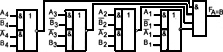
\includegraphics[height = 4\baselineskip]{./assets/02.png}
			\caption{Схема порівняння двох слів на рівність}
			\label{fig:comparator-schematic-02}
			\end{figure}
			
			\begin{table}[!htbp]
			\centering
				\begin{tabular}{llr}
					\toprule
						$A$ & $B$ & $F_{A = B}$ \\
					\midrule
						0101 & 0101 & \\
						1111 & 1011 & \\
						0110 & 0110 & \\
						1100 & 1101 & \\
						1011 & 1100 & \\
					\bottomrule
				\end{tabular}
			\caption{Значення функції порівняння}
			\label{tab:comparator-datasets-02}
			\end{table}
			
		\subsection{Дослідження схеми порівняння двох трьохрозрядних слів~$A$ і~$B$ на~більше}
			Перетворюємо умову порівняння на більше двох слів~$A$ і~$B$ до вигляду, зручного для реалізації на логічних елементах І—АБО—НІ та НЕ—І:
			\begin{IEEEeqnarray}{rCl}
				F_{A > B} &=& \neg \left( \neg \left( A_3 \land \neg B_3 \lor \neg M_3 \land A_2 \land \neg B_2 \lor \neg M_3 \land \neg M_2 \land A_1 \land \neg B_1 \right) \right) \nonumber\\
				          &=& \neg \left(
							\neg \left(
								\neg \left( A_3 \land \neg B_3 \right)
								\land
								\neg \left( \neg M_3 \land A_2 \land \neg B_2 \right)
								\land
								\neg \left( \neg M_3 \land \neg M_2 \land A_1 \land \neg B_1 \right)
							\right)
						\right).
			\end{IEEEeqnarray}
			
			Збираємо схему порівняння двох слів на більше на логічних елементах І—АБО—НІ та НЕ—І~(рис.~\ref{fig:comparator-schematic-03}) відповідно до виразу. Подаємо на входи схеми порівняння двійкові набори слів~$A$ і~$B$~(табл.~\ref{tab:comparator-datasets-03}), і записуємо значення функції~$F_{A>B}$.
			
			\begin{figure}[!htbp]
			\centering
				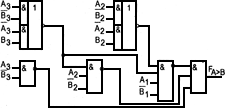
\includegraphics[height = 6\baselineskip]{./assets/03.png}
			\caption{Схема порівняння двох слів на більше}
			\label{fig:comparator-schematic-03}
			\end{figure}
			
			\begin{table}[!htbp]
			\centering
				\begin{tabular}{llr}
					\toprule
						$A$ & $B$ & $F_{A > B}$ \\
					\midrule
						101 & 111 & \\
						111 & 111 & \\
						110 & 011 & \\
						010 & 001 & \\
						001 & 001 & \\
					\bottomrule
				\end{tabular}
			\caption{Значення функції порівняння}
			\label{tab:comparator-datasets-03}
			\end{table}
			
		\subsection{Дослідження схеми контролю парності чотирьохрозрядного слова~$A$}
			Збираємо схему контролю парності чотирьохрозрядного слова~$A$ на~логічних елементах І—АБО—НІ та НЕ—І~(рис.~\ref{fig:comparator-schematic-04}). Подаємо на входи схеми контролю парності двійкові набори слів~(табл.~\ref{tab:comparator-datasets-04}) і записуємо значення функцій~$F_1$ і~$F_2$.
			
			\begin{figure}[!htbp]
			\centering
				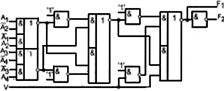
\includegraphics[height = 6\baselineskip]{./assets/04.png}
			\caption{Схема контролю парності}
			\label{fig:comparator-schematic-04}
			\end{figure}
			
			\begin{table}[!htbp]
			\centering
				\begin{tabular}{llrr}
					\toprule
						$A$ & $V$ & $F_1$ & $F_2$\\
					\midrule
						1111 & 0 & & \\
						1011 & 0 & & \\
						1001 & 1 & & \\
						1110 & 1 & & \\
					\bottomrule
				\end{tabular}
			\caption{Значення функцій~$F_1$ і~$F_2$}
			\label{tab:comparator-datasets-04}
			\end{table}
			
	\section{Висновок}
		Під час виконання даної лабораторної роботи ми вивчили логіку роботи, принципи побудови й синтезу схем порівняння (компараторів) та контролю парності. Визначили основні характеристики схем порівняння й контролю парності на інтегральних мікросхемах.
\end{document}